% =============================================================================
%  fig_fault_current_model.tex
%  Schematic decomposition of the three-component fault current model
%  Shows: AC steady-state + decaying AC envelope + DC offset
% =============================================================================
\documentclass[tikz, border=8pt]{standalone}
\usepackage{tikz}
\usepackage{amsmath,amssymb}
\usetikzlibrary{arrows.meta, positioning, calc, decorations.pathreplacing,
                backgrounds, shapes.geometric}

\definecolor{acssC}  {RGB}{ 31, 119, 180}   % AC steady-state — blue
\definecolor{acsubC} {RGB}{214,  39,  40}   % AC subtransient — red
\definecolor{dcC}    {RGB}{ 44, 160,  44}   % DC offset — green
\definecolor{totC}   {RGB}{ 80,  80,  80}   % Total — dark grey
\definecolor{envC}   {RGB}{214,  39,  40}   % Envelope

\tikzset{
  axis/.style = {-{Stealth[length=5pt]}, line width=0.8pt, color=black!70},
  wave/.style = {line width=1.1pt},
  lbl/.style  = {font=\footnotesize},
  ann/.style  = {font=\scriptsize, align=center, color=gray!70!black},
  brace/.style= {decorate, decoration={brace, amplitude=5pt, raise=3pt},
                 color=gray!60, line width=0.7pt},
}

\begin{document}
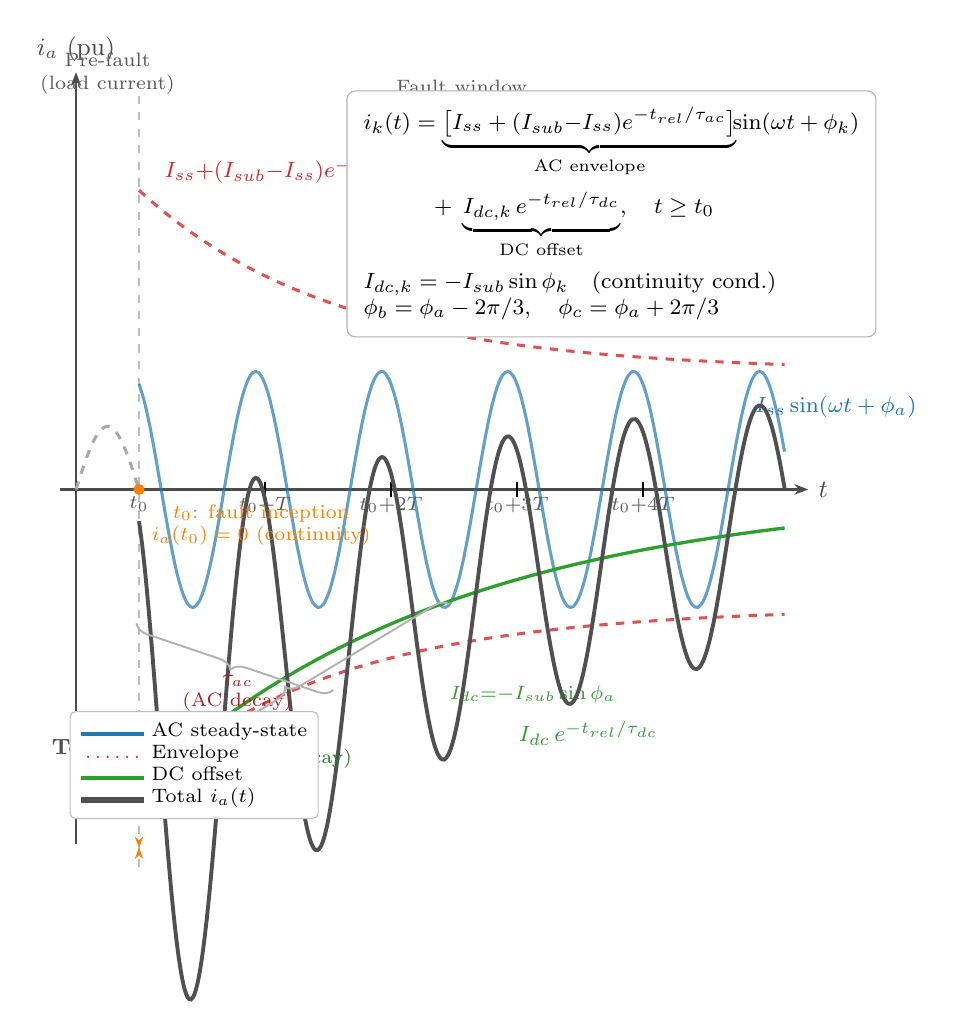
\begin{tikzpicture}

% ---- Coordinate system ------------------------------------------------------
% Time axis: 0..8 cm  (represents ~0 to 0.16 s at 50 Hz, 4 cycles shown)
% Current axis: -3.5..+5 cm (pu)

\def\Tw{9.0}   % width
\def\Th{4.5}   % half-height (total = 2*Th)
\def\t0{0.8}   % fault inception x-coord (cm)
\def\om{3.14159} % omega normalized so 1 period = 2cm

% Axes
\draw[axis] (-0.2, 0) -- (\Tw+0.3, 0) node[right, font=\small] {$t$};
\draw[axis] (0, -\Th) -- (0, \Th+0.8) node[above, font=\small] {$i_a$ (pu)};

% Tick marks on time axis
\foreach \x/\lbl in {0/$t_0$, 2/$t_0{+}T$, 4/$t_0{+}2T$, 6/$t_0{+}3T$, 8/$t_0{+}4T$}
  \draw ({\t0+\x*0.8}, -0.1) -- ({\t0+\x*0.8}, 0.1)
        node[below=2pt, ann] {\lbl};

% Pre-fault region label
\draw[dashed, gray!50, line width=0.6pt] (\t0, -\Th-0.3) -- (\t0, \Th+0.5);
\node[ann, above] at (\t0/2, \Th+0.4) {Pre-fault\\(load current)};
\node[ann, above] at ({(\t0+\Tw)/2}, \Th+0.4) {Fault window};

% --- Pre-fault sinusoid (small amplitude load current) -----------------------
\draw[wave, color=totC!50, dashed]
  plot[domain=0:\t0, samples=40, smooth]
  (\x, {0.8*sin(deg(\om*\x/0.8))});

% --- Drawn with pgf math: parametric curves inside fault window --------------
% We draw component by component using plot expressions

% Parameters (normalized):
%   I_ss  = 1.5 (steady-state amplitude, pu, scaled for display)
%   I_tr  = 2.5 (transient amplitude)
%   I_sub = 3.8 (subtransient amplitude)
%   tau_ac = 2.5 cm (AC decay)
%   tau_dc = 4.0 cm (DC decay)
%   phi_a = pi/2 (maximum asymmetry)

\def\Iss{1.5}
\def\Isub{3.8}
\def\Itr{2.5}
\def\tauac{2.5}
\def\taudc{4.0}

% AC steady-state component  i_ss(t) = I_ss * sin(wt + phi)
\draw[wave, color=acssC, opacity=0.7]
  plot[domain=0:{(\Tw-\t0)}, samples=120, smooth]
  ({\t0+\x}, {\Iss * sin(deg(\om * \x / 0.8 + 90))});
\node[lbl, color=acssC, right] at ({\Tw-0.5}, {\Iss*0.7})
  {$I_{ss}\sin(\omega t + \phi_a)$};

% AC envelope upper/lower (subtransient decaying to steady-state)
\draw[wave, color=envC, dashed, opacity=0.8]
  plot[domain=0:{(\Tw-\t0)}, samples=80, smooth]
  ({\t0+\x}, {(\Iss + (\Isub-\Iss)*exp(-\x/\tauac))});
\draw[wave, color=envC, dashed, opacity=0.8]
  plot[domain=0:{(\Tw-\t0)}, samples=80, smooth]
  ({\t0+\x}, {-(\Iss + (\Isub-\Iss)*exp(-\x/\tauac))});
\node[lbl, color=envC, right] at ({\t0+0.2}, {\Isub+0.25})
  {$I_{ss}{+}(I_{sub}{-}I_{ss})e^{-t_{rel}/\tau_{ac}}$};

% DC offset  i_dc(t) = I_dc * exp(-t/tau_dc),  I_dc = -I_sub*sin(phi) = -I_sub
\draw[wave, color=dcC, line width=1.2pt]
  plot[domain=0:{(\Tw-\t0)}, samples=80, smooth]
  ({\t0+\x}, {-\Isub * exp(-\x/\taudc)});
\node[lbl, color=dcC, right] at ({5.5}, {-3.1})
  {$I_{dc}\,e^{-t_{rel}/\tau_{dc}}$};
\node[ann, color=dcC] at ({5.8}, {-2.6})
  {$I_{dc}{=}{-}I_{sub}\sin\phi_a$};

% Total current (AC + DC)
\draw[wave, color=totC, line width=1.4pt]
  plot[domain=0:{(\Tw-\t0)}, samples=200, smooth]
  ({\t0+\x},
   {((\Iss + (\Isub-\Iss)*exp(-\x/\tauac)) * sin(deg(\om*\x/0.8+90)))
    + (-\Isub * exp(-\x/\taudc))});
\node[lbl, color=totC, left] at ({\t0+0.5}, {-\Isub+0.5})
  {\textbf{Total} $i_a(t)$};

% ---- Annotations: time constants -------------------------------------------
% tau_ac brace
\draw[brace]
  ({\t0+\tauac}, {-(\Iss + (\Isub-\Iss)*exp(-1.0))-0.1}) --
  ({\t0}, {-\Iss-0.1})
  node[midway, below=6pt, ann, color=envC!80!black]
  {$\tau_{ac}$\\(AC decay)};

% tau_dc brace on DC curve
\draw[brace, decoration={brace, mirror, amplitude=5pt, raise=3pt}]
  ({\t0+\taudc}, {-\Isub*exp(-1.0)-0.15}) --
  ({\t0}, {-\Isub-0.15})
  node[midway, below=6pt, ann, color=dcC!80!black]
  {$\tau_{dc}$\\(DC decay)};

% Fault inception marker
\draw[{Stealth[length=4pt]}-{Stealth[length=4pt]},
      color=orange, line width=0.7pt]
  (\t0, {-\Th-0.05}) -- (\t0, {-\Th-0.05});
\fill[orange] (\t0, 0) circle (2pt);
\node[ann, color=orange, below right=2pt and 1pt of {(\t0,0)}]
  {$t_0$: fault inception\\$i_a(t_0)=0$ (continuity)};

% ---- Model equation box -----------------------------------------------------
\node[draw=gray!60, fill=white, rounded corners=3pt, inner sep=6pt,
      align=left, font=\footnotesize] at (6.8, 3.5)
{$i_k(t) = \underbrace{\bigl[I_{ss} + (I_{sub}{-}I_{ss})e^{-t_{rel}/\tau_{ac}}\bigr]}_{\text{AC envelope}}\!\!\sin(\omega t + \phi_k)$\\[4pt]
$\quad\quad\quad +\;\underbrace{I_{dc,k}\,e^{-t_{rel}/\tau_{dc}}}_{\text{DC offset}},\quad t\geq t_0$\\[4pt]
$I_{dc,k} = -I_{sub}\sin\phi_k$\quad (continuity cond.)\\
$\phi_b = \phi_a - 2\pi/3,\quad\phi_c = \phi_a + 2\pi/3$};

% ---- Legend -----------------------------------------------------------------
\node[draw=gray!50, fill=white, rounded corners=2pt, inner sep=4pt,
      align=left, font=\scriptsize] at (1.5, -3.5)
{
  \textcolor{acssC}{\rule{0.8cm}{1.5pt}}\ AC steady-state\\
  \textcolor{envC}{\makebox[0.8cm]{\dotfill}}\ Envelope\\
  \textcolor{dcC}{\rule{0.8cm}{1.5pt}}\ DC offset\\
  \textcolor{totC}{\rule{0.8cm}{2pt}}\ Total $i_a(t)$
};

\end{tikzpicture}
\end{document}
